\chapter{Généralités sur la méthode de champ de phase et le modèle de Cahn-Hilliard mis en \oe uvre} \label{chap:2}
Ce deuxième chapitre résume l'ensemble des notions théoriques liées à la méthode champ de phase. Le couplage avec l'hydrodynamique est présenté puis une description analytique de l'énergie ainsi que les principales hypothèses du modèle sont introduites. 
\section{Méthodes de traitement des interfaces et champ de phase}

%Le traitement numérique efficace des interfaces représente un enjeu majeur de la simulation numérique tant les applications faisant intervenir des interfaces sont importantes. On différencie les méthodes de suivi d'interface des méthodes de capture d'interface. Les méthodes de suivi d'interface suivent des marqueurs placés sur l'interface au cours du temps, la position de l'interface est alors explicite. Les méthodes de capture d'interface quant à elle suivent implicitement l'interface au travers de l'évolution de variables supplémentaires. De nombreuses méthodes existent, on présente ici les principales :
%\begin{itemize}
%	\item[$\bullet$] \textit{\textbf{Volume of fluid (VOF) : }} Cette méthode utilise un maillage fixe découpé en cellule représentant des volumes. On associe alors à chacune de ces cellules une fraction volumique de fluide, cette proportion est alors résolue au cours du temps et la position de l'interface peut être reconstruite. Cette reconstruction a pour désavantage de ne fournir que peu d'informations viables sur l'interface. Cette méthode reste donc peu précise et est également difficile à mettre en \oe uvre en trois dimensions.
%	\item[$\bullet$] \textit{\textbf{Méthode Level-Set (LS) : }}	Cette méthode repose sur la résolution implicite de l'interface au travers de la résolution d'une fonction auxiliaire dite fonction ligne de niveau, généralement la distance signée à l'interface. Cette fonction se doit d'admettre une valeur nulle à l'interface, ainsi au travers de la résolution d'une équation d'advection sur cette fonction ligne de niveau, l'interface est résolue. Cette méthode convient pour les problèmes à fort changement topologique mais présente le désavantage d'être non-conservative.
%	\item[$\bullet$]\textit{\textbf{Arbitrary Lagrangian-Eulerian (ALE) : }} La méthode repose sur une double description lagrangienne (maillage mobile) et eulérienne (maillage fixe), à chaque itération temporelle, le maillage autour de l'interface est reconstruit pour s'adapter à la forme de l'interface, ainsi chaque maille contient uniquement un fluide. L'ensemble de ces propriétés rend la méthode très précise mais difficile à mettre en \oe uvre en trois dimensions.
%	\item[$\bullet$]\textit{\textbf{Front-Tracking (FT) : }} La méthode utilise des marqueurs sans masse positionnés sur l'interface transportée suivant une description lagrangienne sur un maillage eulérien fixe. Ainsi les équations de Navier-Stokes sont résolues sur un maillage fixe tandis que l'équation régissant la position de l'interface est résolue sur un maillage mobile. La principale difficulté réside dans le choix des opérateur de communication entre les deux maillages. Cette méthode nécessite l'implémentation d'algorithme pour les cas de coalescence et rupture d'interface et possède comme désavantage de ne pas être conservative.
%\end{itemize}

De nombreuses méthodes (et combinaison de méthodes) existent pour traiter les problèmes diphasique \cites{mirjalili_interface-capturing_nodate,boniou_comparison_2022}. Par exemple, pour le suivi d'interface, la méthode de Front-Tracking (FT) utilise des marqueurs sans masse positionnés sur l'interface transportée suivant une description lagrangienne sur un maillage eulérien fixe. Ainsi, les équations de Navier-Stokes sont résolues sur un maillage fixe tandis que l'équation régissant la position de l'interface est résolue sur un maillage mobile. La principale difficulté réside dans le choix des opérateurs de communication entre les deux maillages. Cette méthode nécessite l'implémentation d'algorithme pour les cas de coalescence et rupture d'interface et possède comme désavantage de ne pas être conservative. Pour ce qui est du suivi d'interface, la méthode la plus commune est la méthode Volume of fluid (VOF) avec reconstruction géométrique de l'interface. Elle se base sur un maillage eulérien fixe et le suivi des fractions volumiques des différentes phases dans chacune des mailles à partir desquelles l'interface est reconstruite maille par maille (typiquement, de manière linéaire). Cette méthode présente l'avantage d'être conservative et robuste, mais sa mise en \oe uvre est complexe en trois dimensions et sa représentation de l'interface est discontinue d'une maille à l'autre.


Dans les deux précédentes méthodes, l'interface suivie ou reconstruite est une surface sans épaisseur (interface raide). Il existe une autre classe de méthodes dite d'interface diffuse à laquelle les méthodes de champ de phase appartiennent.
Dans ce second cas l'interface correspond donc à une zone d'épaisseur connue et maîtrisée où cohabitent les deux phases, les gradients à l'interface étant finis le traitement numérique est alors facilité. Ce concept d'interface diffuse date du XIX$^{\text{ème}}$siècle et est introduit par Van Der Walls \cite{rowlinson_translation_1979}. Ces deux paradigmes sont présentés en Figure \ref{fig:diffuseinterface}.
\begin{figure}[H]
	\centering
	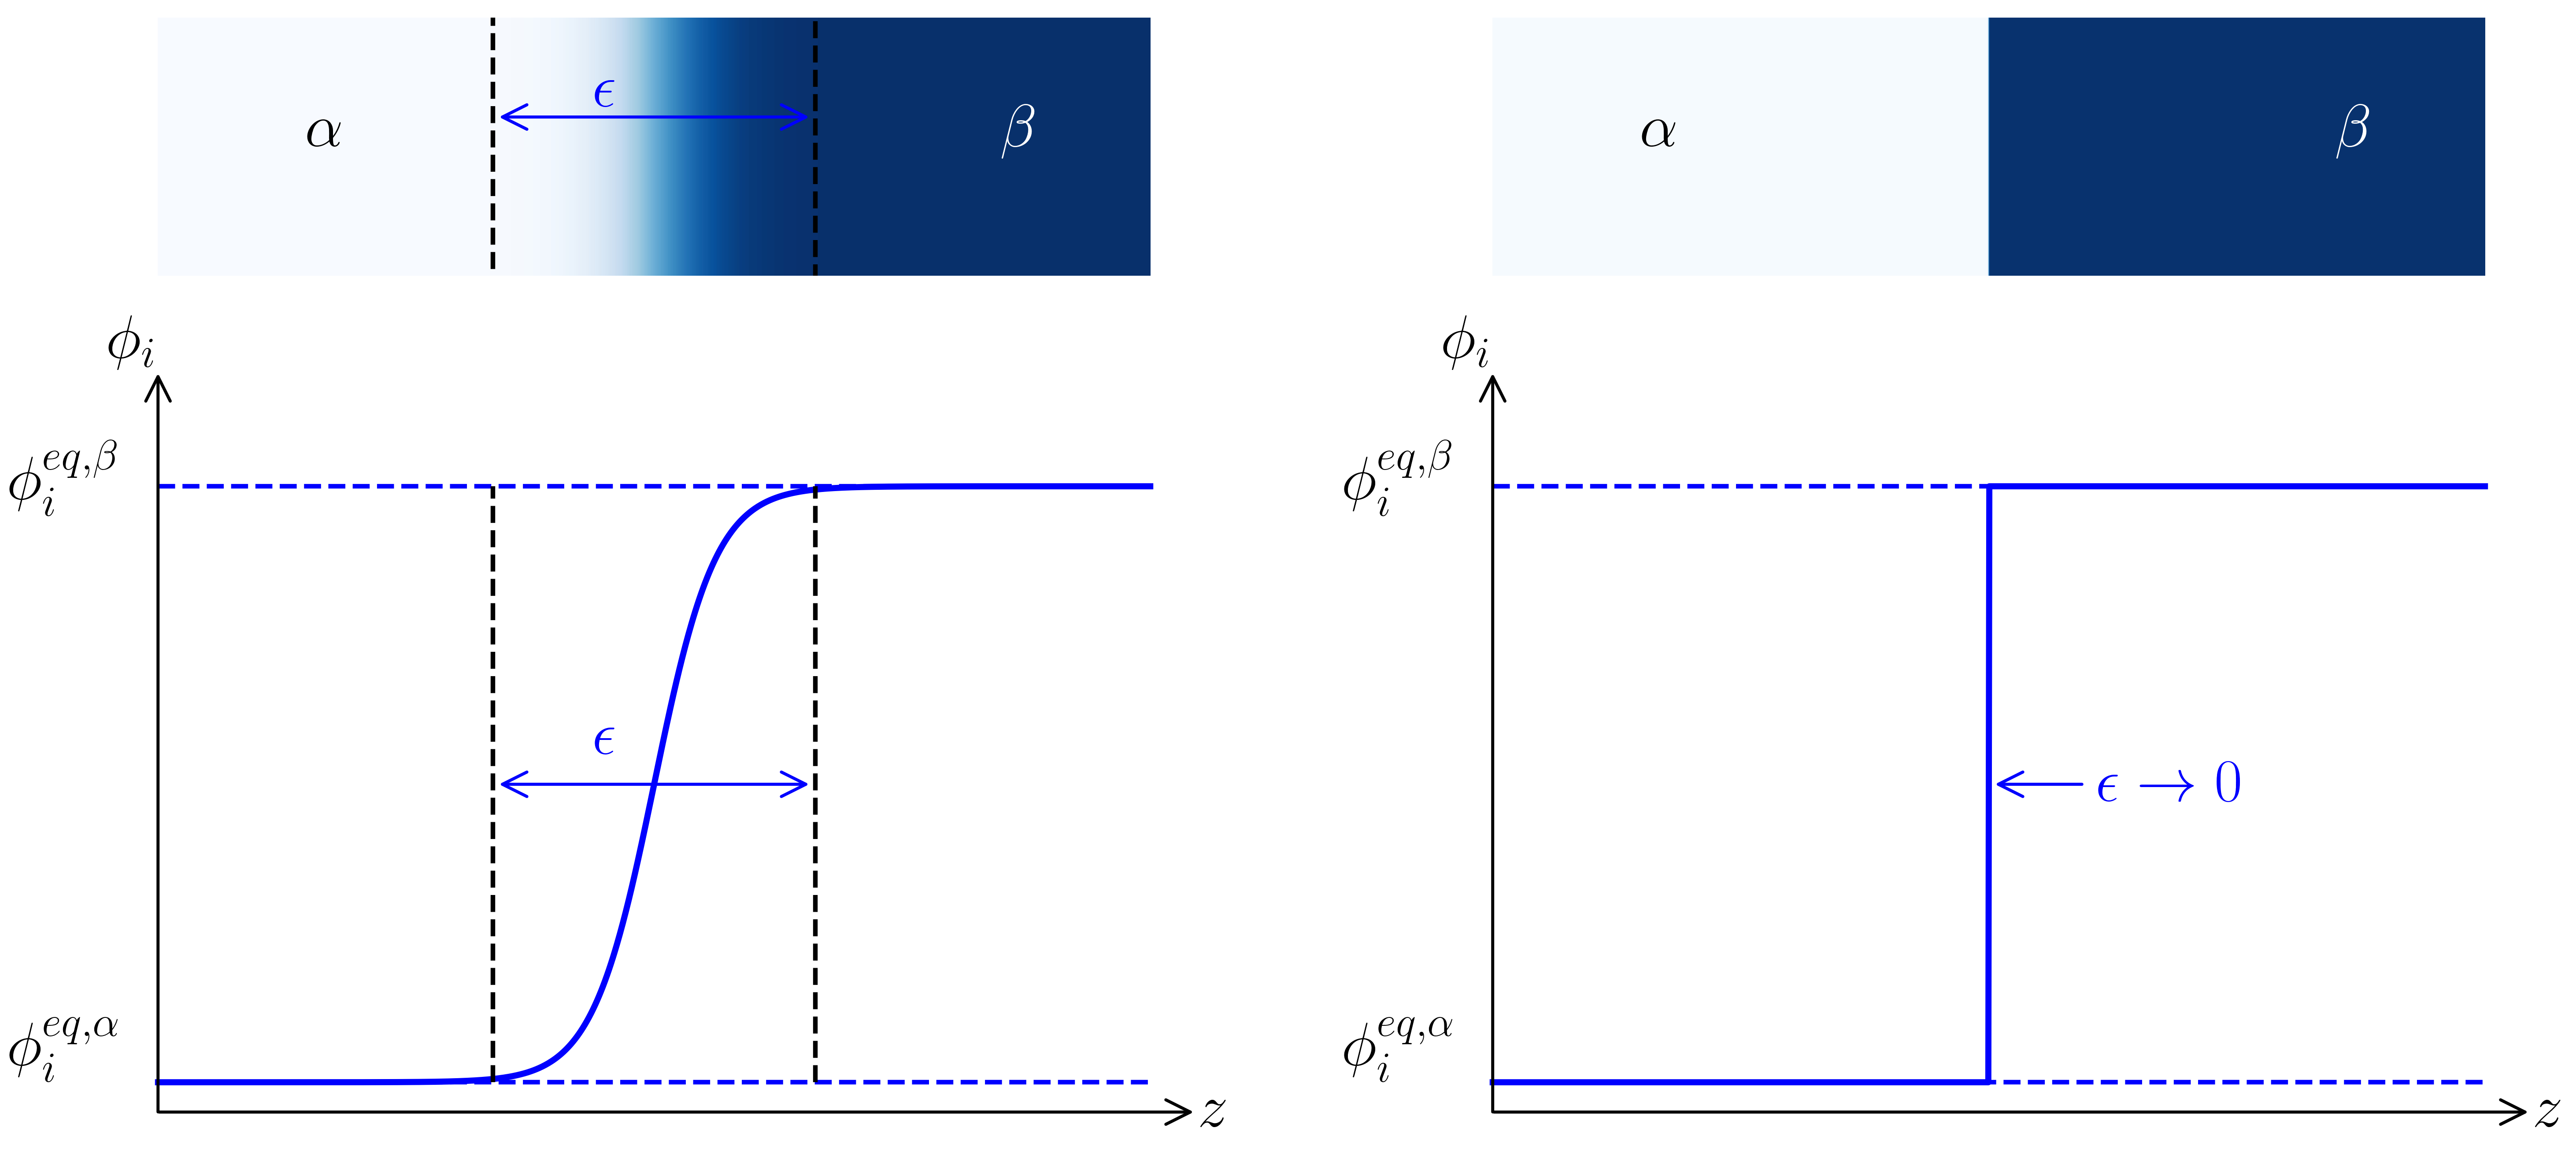
\includegraphics[width=0.7\linewidth]{figure/diffuse_interface}
	\caption{Comparaison entre une interface diffuse (à gauche) et une interface raide (à droite)}
	\label{fig:diffuseinterface}
\end{figure} 
Le concept d'interface diffuse va gagner l'intérêt de la communauté scientifique avec le développement de la méthode champ de phase. En 1950, Ginzburg et Landau proposent une description de l'énergie libre d'un système tenant compte des inhomogénéités spatiales (interfaces) en fonction d'un paramètre d'ordre \cite{landau_physique_1995}. En 1958, Cahn et Hilliard \cite{cahn_free_1958}  introduisent l'utilisation de cette description pour décrire l'évolution de la composition. Ces études sont la base de la méthode champ de phase. En effet la méthode champ de phase est basée sur la représentation d'un système au travers d'une fonctionnelle d'énergie libre, la description diffuse de l'interface et le suivi de paramètres d'ordre $\phi$. Dans le cas d'une physique de l'interface complexe, dans notre cas le transfert de masse multicomposant, le fondement thermodynamique de la méthode la rend intéressante. Le LMAG a donc retenu cette méthode pour la modélisation de la stratification d'un bain de corium. La méthode champ de phase est aujourd'hui utilisée dans de nombreux domaines, certains sont présentés en Figure \ref{fig:champphase}.
\begin{figure}[H]
	\centering
	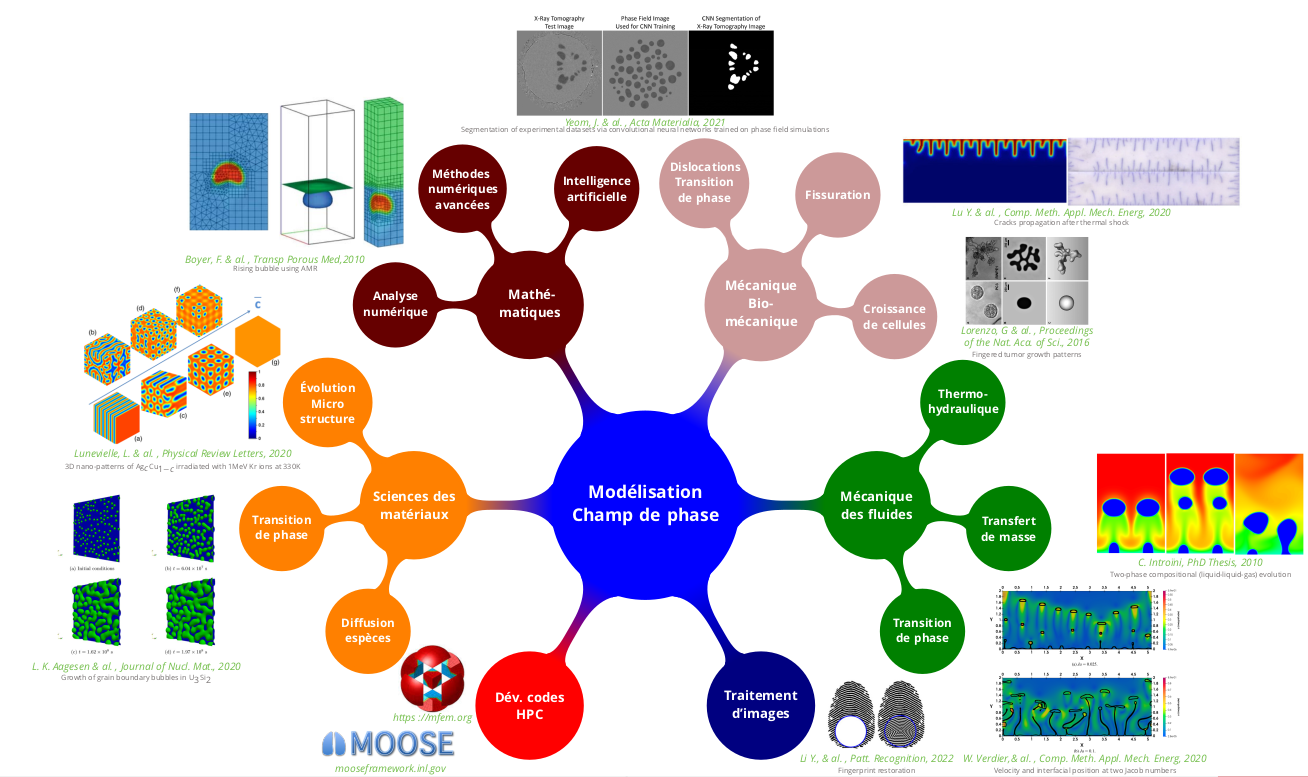
\includegraphics[width=1\linewidth]{figure/champ_phase}
	\caption[Domaine d'application de la méthode champ de phase]{Domaine d'application de la méthode champ de phase, tirée de \cite{introini_suivi_nodate}}
	\label{fig:champphase}
\end{figure} 





\section{Méthode champ de phase conservative, équation de Cahn-Hilliard généralisée}

Dans le cas d'un système à n-composants on note $\{\phi_i\}_{i=1,..n}$ \footnote{Par soucis de simplification, on pourra également utiliser la notation $\{\phi\}$} l'ensemble des paramètres d'ordre du système. Ces paramètres peuvent représenter la concentration, la fraction massique ou d'autres grandeurs.
Comme expliqué précédemment, la méthode de champ de phase repose sur le suivi de ces variables. Ces paramètres d'ordre peuvent être conservés ou non, dans notre étude les paramètres d'ordres sont conservés. De plus, on considère un système fermé. L'utilisation de la concentration comme paramètre d'ordre amène la contrainte supplémentaire :
\begin{equation}
\sum_{i=1}^n \phi_i =1 \Rightarrow \phi_n =1 - \sum_{i=1}^{n-1} \phi_i
\end{equation} 
Ainsi pour un mélange à $n$ composants, cette loi de fermeture permet de décrire l'ensemble du système en suivant l'évolution d'uniquement $n-1$ composants. Dans certains cas, le système peut également être décrit avec des variables non conservées telles que des indicatrices de phases ou des grandeurs liées à des réactions chimiques. Le comportement de ces variables est alors régi par des équations de réaction-diffusion dites d'Allen-Cahn, non présentée ici. Dans le cadre de variables conservées les équations de Cahn-Hillard pour $n$ composants, avec $i\in \{1,..,n-1 \}$ s'écrivent sous la forme :
\begin{equation}
	\cfrac{\partial \phi_i}{\partial t} + \left(\mathbf{u} \cdot \nabla\right) \phi_i =  \nabla \cdot \left(\sum_{j=1}^{n-1}{\mathcal{M}_{ij}} \nabla\left( \frac{\delta \mathbb{F}}{\delta \phi_j}\right) \right) 
\end{equation}
avec : $\mathcal{M}_{ik}$ les coefficients de mobilité (paramètre cinétique),  $\phi_i$ le paramètre d'ordre, $\mathbf{u}$ la vitesse et $\mathbb{F}$ une fonctionnelle de Ginzburg-Landau généralisée \cite{cardon_modelisation_2016} définie tel que : 
 \begin{equation}
\mathbb{F}[\{\phi\}] = \int_{\mathcal{V}}\lambda\tilde{g}^{}(\{\phi\},\mathbf{x},t)+ \sum_{i=1}^{n-1}\sum_{j=1}^{n-1}\cfrac{1}{2}\kappa_{ij}\nabla \phi_i \cdot \nabla \phi_j dV
\end{equation}
Avec $\mathbf{x}$ le vecteur position et $V$ le volume.
Le premier terme représente la densité d'énergie liée aux valeurs locales de composition, traduisant l'équilibre des phases ainsi que leurs existences ou coexistences. Pour deux phases $\alpha$ et $\beta$, on rappelle les conditions données par l'équilibre thermodynamique \cite{kim_phase-field_1999} :
\begin{subequations}
	\label{eq:all}
	\begin{empheq}[left={\empheqlbrace\,}]{align}
		&\lambda\left.\frac{\partial \tilde{g}^{}}{\partial \phi_i}\right|_{\phi_i^{\alpha,eq}} = \lambda\left.\frac{\partial \tilde{g}^{}}{\partial \phi_i}\right|_{\phi_i^{\beta,eq}} = \tilde{\mu}_i^{eq} \\
& 		\lambda\tilde{g}^{\alpha,eq} - \sum_{i=1}^{n-1}\tilde{\mu}_i^{eq}\phi_i^{\alpha,eq} = 	\lambda\tilde{g}^{\beta,eq} - \sum_{i=1}^{n-1}\tilde{\mu}_i^{eq}\phi_i^{\beta,eq}
	\label{eq:sapparenteGP}
	\end{empheq}
\end{subequations}
$\tilde{\mu}_i^{eq}$ représente un potentiel de diffusion de l'élément $i$ à l'équilibre. L'équation \ref{eq:sapparenteGP} s'apparente à l'égalité du "grand potentiel" thermodynamique. \\
Le second terme représente la contribution des interfaces, le coefficient $\kappa_{ij}$, dit coefficient de gradient, tient compte du coût énergétique engendré par l'interface, par la suite ce paramètre pourra être relié à la tension de surface. \\
%Dans le cas binaire il est possible de décrire géométriquement l'ensemble des variables : 
%\begin{figure}[H]
%	\centering
%	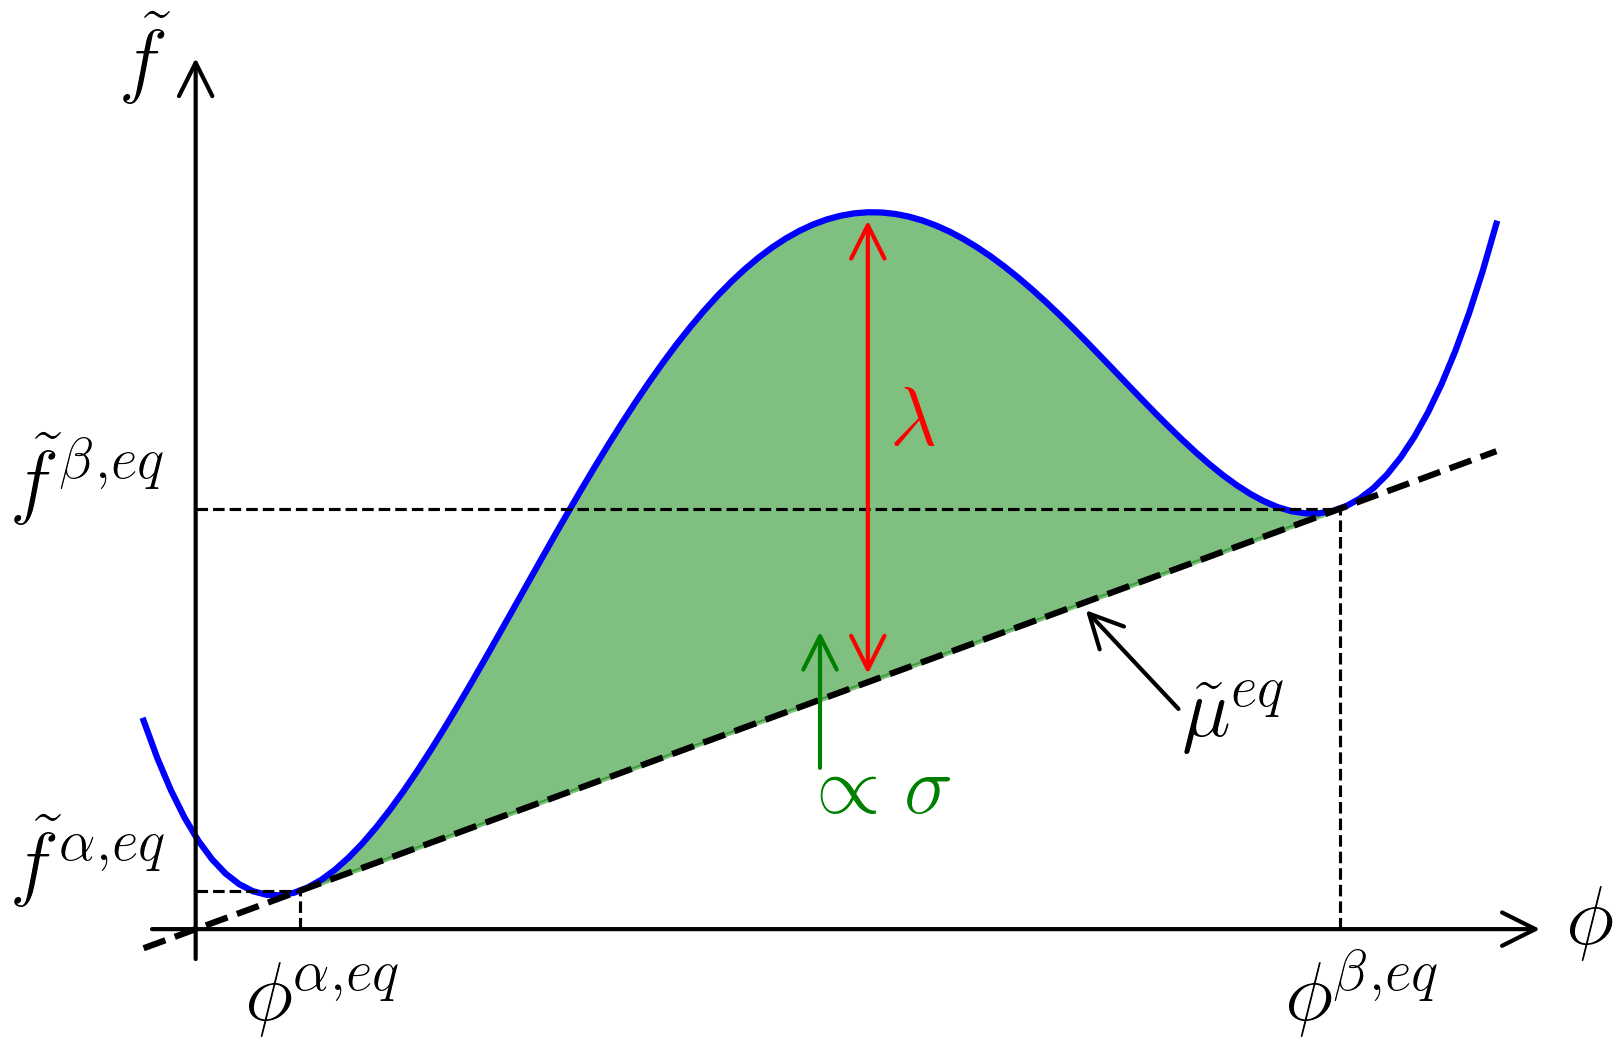
\includegraphics[width=0.45\linewidth]{figure/fig_NRJ}
%	\caption{Description de l'énergie libre pour un système binaire}
%	\label{fig:fignrj}
%\end{figure}
Finalement la dérivée variationnelle de cette fonctionnelle d'énergie libre peut être définie comme un potentiel de diffusion $\tilde{\mu}$: 
\begin{equation}\label{eq_potentiel}
	\frac{\delta \mathbb{F}}{\delta \phi_j} =\lambda \frac{\partial \tilde{g}}{\partial \phi_j} -\sum_{k=1}^{n-1} \kappa_{jk} \Delta \phi_k = \tilde{\mu}_j
\end{equation}
avec $\lambda$ un paramètre d'\textit{upscaling} numérique ajouté pour permettre l'augmentation de l'épaisseur de l'interface au-delà de son épaisseur physique tout en conservant la tension de surface à l'équilibre. Cet élargissement de l'interface permet d'utiliser des maillages réalistes compte tenu des capacités de calcul actuelles. \\
Le potentiel de diffusion peut être relié au potentiel chimique classique tel que :
%\begin{equation}
%	\tilde{\mu}_i = \frac{\lambda}{V_m}\left(\mu_i - \mu_n\right)
%\end{equation}
\begin{subequations}
	\begin{empheq}[left={\empheqlbrace\,}]{align}
	&\tilde{\mu}_i = \frac{\lambda}{V_m} \hat{\mu}_i \\
		& \hat{\mu}_i = \mu_i - \mu_n
	\end{empheq}
\end{subequations}
Avec $\tilde{\mu}_i$ (en J.m$^{-3}$) le potentiel de diffusion volumique de l'élément $i$, $\hat{\mu}_i$ (en J.mol$^{-1}$) le potentiel de diffusion molaire, ${\mu}_i$ (en J.mol$^{-1}$) le potentiel chimique de l'élément $i$ et $V_m$ le volume molaire supposé constant dans tout le système. \footnote{Dans le cadre de ce rapport on note $\tilde{.}$ les grandeurs volumiques}\\
%Le potentiel chimique étant classiquement définit tel que :
%\begin{equation}
%	\mu_i = \left.\frac{\partial G}{\partial n_i}\right|_{P,T,n_{j\neq i }} = \left.\frac{\partial F}{\partial n_i}\right|_{V,T,n_{j\neq i }}
%	  \textrm{                        où           } F = V_m f_0
%\end{equation}
%Avec $F$ (resp. $G$) l'énergie libre d'Helmotz (resp. Gibbs) (en J) et $n_i$ la quantité de matière de l'élément $i$ (en mol). Dans notre cas on se place dans une transformation isobare et isotherme, on privilégiera donc l'énergie de libre de Gibbs.
Dans le cas où $\doubleoverline{\kappa}$ = $\doubleoverline{0}$ on retrouve une équation d'advection-diffusion classique, dans le cas contraire on obtient une équation d'ordre 4. Pour un système binaire le gradient d'énergie et le paramètre d'\textit{upscaling} peuvent être déterminés analytiquement. Dans le cas d'une modélisation à n-composants cette approche analytique ne fonctionne plus (à l'exception de certains cas particuliers, par exemple le cas ternaire présenté dans \cite{lapuerta_echanges_2006}). Ainsi une des principales difficultés de la mise en place de la méthode champ de phase dans les cas n-aire est l'obtention de ces paramètres.
Dans la suite de ce travail nous utiliserons une proposition de paramétrage introduite par \cite{rasolofomanana_numerical_nodate} et présentée en annexe \ref{ann:parametrage}. Cette paramétrisation permet de déterminer les paramètres d'\textit{upscaling} $\lambda$ et le gradient d'énergie $\bm{\bar{\bar{\kappa}}}$ en fonction des paramètres physiques du système, la tension de surface $\sigma$ et l'épaisseur d'interface $\epsilon$. Ce paramétrage est construit de façon à être consistant vis-à-vis d'un système binaire.
\begin{subequations}
	\label{eq:all}
	\begin{empheq}[left={\empheqlbrace\,}]{align}
	&\bm{\bar{\bar{\kappa}}} = \frac{\sigma \epsilon}{\xi_1 \xi_2}\delta_{ij}
	\label{eq:1} \\
	&\lambda=\frac{\xi_2 \sigma}{2\epsilon\xi_1}
	\label{eq:2}
	\end{empheq}
\end{subequations}
avec $\xi_1 ,\xi_2$ deux constantes dépendantes de la description thermodynamique adoptée, $\delta_{ij}$ le symbole de Kronecker.
\section{Couplage avec les équations de Navier-Stokes incompressible}
Dans le cadre de cette étude, les équations de Cahn-Hilliard sont couplées aux équations de conservation de masse et de quantité de mouvement incompressible. Kim J. \cite{kim_phase-field_2012} présente un modèle \textit{one fluid}. Les équations de Navier-Stokes s'écrivent sous la forme :
\begin{subequations}
	\label{eq:all}
	\begin{empheq}[left={\empheqlbrace\,}]{align}
	&\nabla \cdot \mathbf{u} = 0\\
	&\rho\left(\{\phi_i\}\right) \left (\frac{\partial \mathbf{u}}{\partial t} + (\mathbf{u} \cdot {\nabla})\mathbf{u}\right) = -{\nabla} P +\eta \Delta \mathbf{u}+\sum_{i=1}^{n-1} \tilde{\mu}_i{\nabla} \phi_i + \rho\left(\{\phi_i\}\right) \mathbf{g}
	\end{empheq}
\end{subequations}
avec $\mathbf{u}$ la vitesse, $P$ la pression, $\mathbf{g} = \{ 0,0,-g\}^T $, $\eta$ la viscosité dynamique supposée constante, $\rho\left(\{\phi_i\}\right)$ la masse volumique. \\
%L'hypothèse du volume molaire constant nous impose que la loi de densité soit une combinaison linéaire des masses volumiques des corps purs que l'on écrit sous la forme : 
%\begin{equation} \label{eq:boussi}
%	\rho\left(\{\phi_i\}\right) = \rho(\phi_n)\left(1+\sum_{i=1}^{n-1}\beta_i \phi_i\right)
%\end{equation}
%Les paramètres $\beta_i$ sont à déterminer en fonction du système étudié, $\rho(\phi_n)$ correspond à une masse volumique de référence, généralement celle du solvant.
L'hypothèse du volume molaire constant nous impose que la loi de densité soit une combinaison linéaire des masses volumiques des corps purs. Ainsi un développement de Taylor autour d'une densité de référence associée à un profil de concentration $\{\phi^*_i\}_{i=1,..,n-1}$.
\begin{equation} \label{eq:taylor}
	\rho(\{\phi_i\}) = \rho(\{\phi_i^*\}) + \sum_{i=1}^{n-1} (\phi_i - \phi_i^*)\left.\frac{\partial \rho}{\partial \phi_i}\right|_{\phi_j\neq \phi_i} + o(\phi_i - \phi_i^*)
\end{equation}
Ainsi en négligeant $o(\phi_i - \phi_i^*)$ l'équation \ref{eq:taylor} peut se réécrire, en introduisant la notation $\rho(\{\phi_i^*\}) = \rho^*$ :
\begin{subequations}
	\label{eq:boussinesq}
	\begin{empheq}[left={\empheqlbrace\,}]{align}
	\label{eq:boussiref}
	&\rho\left(\{\phi_i\}\right) = \rho^*\left(1+\sum_{i=1}^{n-1}{\beta}_i (\phi_i-\phi_i^*)\right)\\
	&{\beta}_i = \frac{1}{\rho^*}\left.\frac{\partial \rho}{\partial \phi_i}\right|_{\phi_j\neq \phi_i}
	\end{empheq}
\end{subequations}
Avec $\beta$ les coefficients de dilatation à déterminer en fonction des espèces du système. Pour la suite de ce travail, nous choisissons de poser $\{\phi_i^*\} = \{0\}$, tel que la masse volumique de référence soit la masse volumique du corps pur du $n$-ième élément du système. Pour la suite de l'étude nous utiliserons une densité constante et égale à $\rho^*$ dans tous les termes à l'exception du terme de flottabilité. On utilise également une pression corrigée noté $P^*$ déterminée tel que :
\begin{equation}
	P^* = P - \rho^* (\mathbf{g} \cdot \mathbf{x})
\end{equation}
\section{Paysage thermodynamique analytique}
\subsection{Introduction d'un pseudo-grand potentiel}
L'objectif présenté dans \cite{rasolofomanana_numerical_nodate} est d'obtenir une formulation analytique du terme homogène de la fonctionnelle de Ginzburg-Landau. Dans le cas binaire, cette contribution est de la forme d'un double puits, généralement un polynôme de degré 4.
L'objectif est de généraliser ce double puits pour un système n-aire, ainsi un pseudo grand potentiel correspondant à la hauteur énergétique nécessaire pour changer de minimum d'énergie \cite{cardon_modelisation_2016} est introduit.
\begin{equation}
\Omega^{\star} =\Omega - \Omega^{eq} =  {g} - \sum_i \hat{\mu}_i^{eq}\phi_i - \left(  {g}^{eq} -  \sum_i \hat{\mu}_i^{eq}\phi_i^{eq} \right) 
\label{eq:grandpotent}
\end{equation}
avec ${g}^{}$ l'énergie libre de Gibbs (J.mol$^{-1}$)\footnote{En utilisant l'hypothèse du volume molaire constant il est possible d'écrire $\tilde{g} = {g}/{V_m}$}, utilisé comme grandeur d'intérêt ici puisque le système est supposé isotherme et isobare.
	\subsection{Application pour un cas diphasique ternaire}
Comme présenté au chapitre \ref{chap:1} le cas d'intérêt de l'étude est le corium. Ce système comprend deux phases à l'équilibre et donc deux points d'équilibre distincts.  Ainsi \cite{rasolofomanana_numerical_nodate} introduit une formulation sous la forme d'un double puits de la forme :
\begin{equation}\label{double_puit}
	\Omega^{\star}  = P^{\alpha} \times P^{\beta}
\end{equation}
Où $P^{\alpha}, P^{\beta}$ représentent deux paraboloïdes correspondant aux deux phases en présence. Dans le cas ternaire, en considérant deux éléments d'intérêt notés 1 et 2 ces paraboloïdes s'écrivent :
\begin{multline}
P^{k}=\left(\frac{\co{\theta^{k}}(\phi_{1}-\phi_{1}^{eq,k}) + \sinus{\theta^{k}}(\phi_{2}-\phi_{2}^{eq,k})}{a_{1}^{k}}\right)^{2}+\\ \left(\frac{-\sinus{\theta^{k}}(\phi_{1}-\phi_{1}^{eq,k}) + \co{\theta^{k}}(\phi_{2}-\phi_{2}^{eq,k})}{a_{2}^{k}}\right)^{2}
\label{eq:paraboloid_general_}
\end{multline}
Avec $k = \{\alpha,\beta\}$ la phase (dispersée ou continue), $a_{1}^k$ (resp. $a_{2}^k$) le demi-petit  (resp. demi-grand) axe, $\theta^k$ l'angle de rotation associé au puits de la phase $k$.\\
Le cas du paysage le plus simple est alors tracé en Figure \ref{fig:landscape}.
\begin{figure}[H]
	\centering
	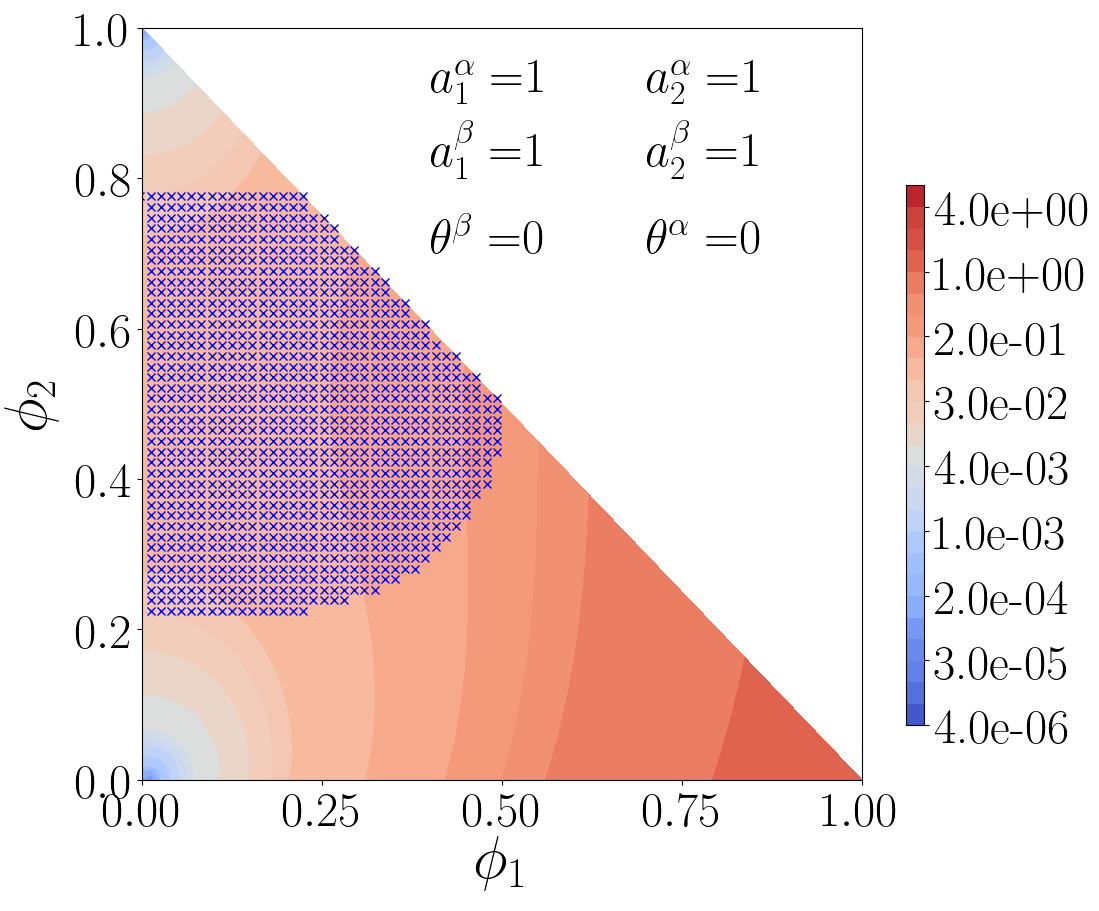
\includegraphics[width=0.6\linewidth]{figure/landscape}
	\caption{Exemple de paysage thermodynamique, la zone bleu représente la zone instable}
	\label{fig:landscape}
\end{figure}
%Les éléments de calculs pour la détermination de la zone instable sont présentés en annexe \ref{ann:stabphase}, cette zone correspond à des compositions pour lesquels le système subit une séparation de phase, ainsi il est primordiale que cette zone n'englobe pas les conditions initiales. Une représentation dans le plan est possible pour le cas ternaire, pour les cas comprenant un nombre plus important de paramètres d'ordre la visualisation semble plus complexe. Ainsi cette formulation possède l'avantage d'éviter un couplage entre le code CFD et un solveur d'équilibre thermodynamique (Open-Calphad par exemple) réduisant significativement le temps de développement. En effet pour les cas ou le paysage est connu il est alors possible de calibrer les paramètres des paraboloïdes pour obtenir une forme analytique proche du paysage réel. Dans le cas d'un paysage inconnu, par manque d'information thermodynamique, ce paysage permet d'avoir une description cohérente pour des simulations qualitatives.

La zone instable correspond à la zone où la séparation de phase a lieu, la détermination de cette zone est obtenue d'après \cite{aursand_spinodal_2017}. \\
Pour le cas du corium, dans \cite{cardon_modelisation_2016} l'énergie libre homogène utilisée pour résoudre l'équation de Cahn-Hilliard était reliée à l'énergie de Gibbs d'une phase liquide construite selon une méthode CALPHAD en utilisant des bases thermodynamiques. Un tel couplage peut considérablement augmenter les temps de calculs en réalisant des calculs de minimisation de l'énergie locale en chaque point du maillage pour chaque pas de temps. La formulation analytique associée à l'équation \ref{eq:grandpotent} permet de s'affranchir de ces difficultés. Par ailleurs, dans le cas d’un système sans données thermodynamiques, cette formulation permet d’obtenir des simulations qualitatives. Dans le cas d’un système complètement décrit thermodynamiquement, cette formulation analytique peut aussi être utilisée pour approcher le paysage thermodynamique donné par une base aux alentours des points d'équilibre \cite{verdier_phase-field_2022} (par une procédure d'ajustement des paramètres).


%On peut dès lors calculer le potentiel de diffusion homogène grâce à la formulation analytique (\ref{double_puit}) :
%\begin{align}
%	\tilde{\mu}_i & \nonumber= \frac{\partial}{\partial \phi_i}\left\lbrace 
%	\Omega^{\star} + \sum_j \tilde{\mu}_j^{eq}\phi_j + \left( {g}^{liq,eq} -  \sum_j \tilde{\mu}_j^{eq}\phi_j^{eq} \right)\right\rbrace \\
%	&\nonumber = \frac{\partial \Omega^{\star}}{\partial \phi_i} + \frac{\partial g^{liq,eq}}{\partial \phi_i} + \sum_j \frac{\partial \tilde{\mu}_j^{eq}\left(\phi_j - \phi_j^{eq}\right)}{\partial  \phi_i}\\
%	\tilde{\mu}_i &=	P^{dis}\frac{\partial P^{cont}}{\partial \phi_i} + P^{cont}\frac{\partial P^{dis}}{\partial \phi_i} + \tilde{\mu}_i^{eq}
%\end{align} 
%%\begin{align*}
%	%& \frac{\partial g^{liq,eq}}{\partial \phi_i} = 0 \\
%		%& \sum_j \frac{\partial \tilde{\mu}_j^{eq}\left(\phi_j - %\phi_j^{eq}\right)}{\partial  \phi_i} = \tilde{\mu}_i^{eq} %+\tilde{\mu}_{j\neq i}^{eq} \frac{\partial \phi_{j\neq i}}{\partial %\phi_i} = \tilde{\mu}_i^{eq}
%%\end{align*}
%L'objectif est alors de déterminer les paramètres des paraboloïdes pour obtenir des résultats consistants thermodynamiquement.


